\documentclass[a4paper,10pt]{article}
\usepackage[utf8]{inputenc}
\usepackage[italian]{babel}
\usepackage{amsmath}
\usepackage{graphicx}

%opening
\title{Relazioni dal laboratorio di calcolo}
\author{Riccardo Iaconelli}

\begin{document}

\maketitle

\begin{abstract}
Durante il Laboratorio di calcolo del terzo anno vengono mostrate alcune tecniche numeriche per la soluzione di problemi comuni in Fisica. In particolare l'attenzione è posta su diverse tecniche per svolgere integrali, sia di tipo deterministico che Monte-Carlo. Il programma si divide in più parti: per cominciare una sezione in cui si investigano tecniche per ridurre l'imprecisione numerica implicita di un calcolatore, dopodiché si studiano imprecisioni e rapidità di diversi algoritmi per il calcolo di integrali, e infine si applicano queste tecniche a problemi fisici. Come ultimo esercizio si implementa il metodo di Runge-Kutta per risolvere numericamente equazioni differenziali.
\end{abstract}
\clearpage

\section{Serie numeriche e precisione floating point}
Questo primo esercizio viene eseguito per mostrare come si possono ridurre eventuali errori di calcolo introdotti dalle normali operazioni aritmetiche.

\subsection{Analisi teorica}
All'interno del calcolatore le cifre non sono rappresentabili con precisione infinita. A causa di ciò, con ogni operazione effettuata è possibile ottenere errori numerici dovuti a due tipi di problemi.
\begin{description}
 \item[Errore di overflow (o underflow)] Questo errore avviene quando il risultato è più grande del massimo numero rappresentabile, o più piccolo del minimo numero rappresentabile.
 \item[Errore di troncamento] Quando operazioni di \textit{shift} comportano errori di arrotondamento.
\end{description}

Per vedere come questo è possibile, studiamo come sono rappresentati i numeri all'interno di un calcolatore.
La rappresentazione all'interno del calcolatore dei numeri floating-point è fissata dallo standard IEEE 754 (1985).
Questa specifica indica che, dato $x$ numero float, viene separato in tre parti (\textit{segno}, \textit{mantissa} ed \textit{esponente}) nel seguente modo:
\begin{equation}
 x= (-1)^\text{\ segno} \cdot\text{mantissa}\cdot 2^{\text{\ esponente}-E}
\end{equation}

Per ottimizzare le oeprazioni, gni numero viene inoltre memorizzato in forma ``normalizzata'', ovvero si ha sempre che
$$\text{mantissa} = 1.\text{frazione}$$
Ad esempio, il numero:
$$0.15625_{10} = 0.00101_2 = 1.01_2 \cdot 2^{-3}$$

In particolare, lo standard definisce due tipi di numeri con differenti precisione e con diverso \textit{bias} ($E$):
\begin{description}
 \item[\texttt{float}] Numeri in singola precisione, che utilizzano 32 bit di memoria. $E = 127$.
 \item[\texttt{double}] Numeri in doppia precisione, che utilizzano 64 bit di memoria. In questo caso, $E=1023$.
\end{description}
I bit utilizzati per la rappresentazione sono così ripartiti:
\begin{center}
\begin{tabular}[center]{c|c|c|c}
 & Segno & Esponente & Frazione \\ 
\hline
float & 1 & 8 & 23\\
\hline
double & 1 & 11 & 52 \\
\end{tabular}
\end{center}

Nel caso appena visto, $0.15625_{10} = 1.01_2 \cdot 2^{-3}$ sarebbe rappresentato in questo modo in un \texttt{float}:
\begin{itemize}
\item $\text{segno}=0$
\item $\text{esponente}=127-3=124=11111000$
\item $\text{frazione}=010000...$
\end{itemize}
Una rappresentazione grafica della memoria utilizzata da un numero \texttt{double} è qui offerta:

% \begin{figure}
%  \centering
\begin{center}
 \includegraphics[scale=0.35]{./images/1000px-IEEE_754_Double_Floating_Point_Format.png}
\end{center}
 % 1000px-IEEE_754_Double_Floating_Point_Format.svg.png: 1000x202 pixel, 72dpi, 35.28x7.13 cm, bb=0 0 1000 202
%  \caption{Una rappresentazione grafica di un numero float}
% \end{figure}
Si nota facilmente che c'è un errore intrinseco nella rappresentazione dei numeri dovuto alla finitezza della memoria utilizzata, non tutti i numeri sono infatti rappresentabili, e il ``gap'' tra un numero e il successivo varia in base all'ordine di grandezza utilizzato. Questo errore aumenta con alcune operazioni, consideriamo ad esempio una somma.

\subsubsection{L'algoritmo di somma}
Quando un calcolatore deve eseguire una somma, procede nel seguente modo:
\begin{itemize}
\item Per prima cosa, vengono confrontati gli esponenti dei due numeri, e viene \emph{shiftato}\footnote{traslato, l'operazione equivalente a dividere o moltiplicare per due} l'esponente del numero più piccolo, fino a che i due esponenti non sono uguali.
\item Vengono a questo punto sommate direttamente le mantisse, seguendo le normali regole del complemento a due.
\item Il numero così ottenuto viene normalizzato, modificando l'esponente di conseguenza
\item Come ultimo passaggio, la mantissa viene arrotondata per rimanere nel numero di bit richiesto. 
\end{itemize}

Da questo processo si vede chiaramente come si ha una grossa perdita di precisione nel caso di somme di numeri di ordini di grandezza molto diversi tra loro. Quando infatti la differenza tra gli esponenti è dell'ordine di grandezza della precisione della mantissa, il contributo del numero più piccolo si perde nell'arrotondamento.

Questo concetto sarà ulteriormente chiarito nel prossimo esercizio.

\subsubsection{La serie di Eulero}
Per mettere in pratica quanto visto finora in teoria, studiamo le somme parziali della serie di Eulero:
$$\sum_{n=1}^\infty \frac{1}{n^2} = \frac{\pi^6}{2} \simeq 1.6449340 $$

Per mettere più in evidenza il problema di arrotondamento, eseguiamo i nostri calcoli utilizzando solamente variabili di tipo \texttt{float}. Notiamo che nell'ordine di grandezza in cui stiamo lavorando ($2^0$) il più piccolo step rappresentabile è dato direttamente dalla precisione della mantissa: $2^{-23}\simeq 1.19\cdot10^{-7}$. Tutti i risultati saranno dunque presentati con sole 7 cifre significative.

\paragraph{Somma crescente}
Proviamo inizialmente a sommare i numeri in ordine crescente, ovvero consideriamo
$$S_k := \sum_{n=1}^k \frac{1}{n^2}$$
Notiamo immediatamente che quando $n^2\simeq2^{24}$, l'operazione di arrotondamento successiva alla somma (potendo utilizzare solo 23 bit per la mantissa, e sommando sempre un numero di ordine di grandezza $2^0$) perda ogni tipo di contributo dei nuovi numeri.

Ci aspettiamo allora che, definito: $$k_\text{critico} := \sqrt{2^{24}} = 4096$$


$\forall k \geq k_\text{critico}$ la somma smetta di crescere, e dunque $S_k = S_{k+1} = ...$.

\paragraph{Somma decrescente}
Per evitare il problema di arrotondamento appena illustrato, possiamo provare a considerare una somma ``inversa'' o decrescente, ovvero definire (con un piccolo abuso di linguaggio):

$$S_k := \sum_{n=k}^1 \frac{1}{n^2}$$

In questo modo, la somma parziale mantiene il più possibile l'ordine di grandezza del nuovo termine da aggiungere, minimizzando il problema di arrotondamento.

\paragraph{Confronto tra i due metodi}
Dopo aver realizzato in C++ due programmi che implementassero quanto appena descritto, rappresentiamo in un grafico (in scala logaritmica) l'errore che si commette con entrambi i metodi e la differenza dal valore vero.
\begin{center}
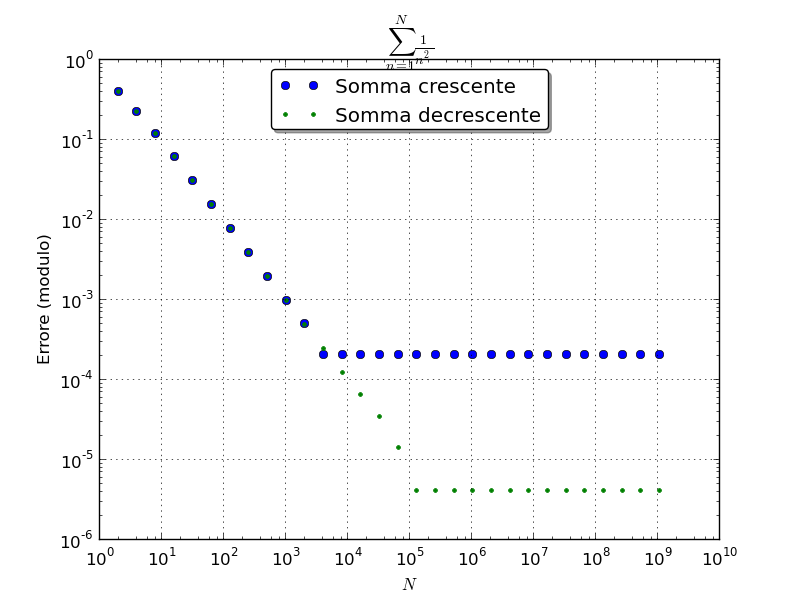
\includegraphics[scale=.55]{../images/serie.png}
\end{center}

Notiamo come l'errore scende drammaticamente utilizzando il metodo della somma decrescente. In particolare, si raggiunge tranquillamente una precisione dell'ordine di $10^{-7}$, come prescriverebbe la teoria. Continunando con le iterazioni si arriva anche a $10^{-8}$, anche se è solo una fluttuazione numerica priva di ogni significatività.

\subsection{Conclusioni}
Abbiamo studiato come la rappresentazione finita dei numeri all'interno di un calcolatore introduca errori ed imprecisioni all'interno dei nostri algoritmi.
Questi errori, se non considerati, possono portare a significativi errori nel computo finale.

Conoscendo bene come funzionano le operazioni di base nel calcolatore, è però possibile con alcuni accorgimenti raggiungere precisioni molto vicine a quelle consentite dalla rappresentazione stessa.

Viene allegato il codice sorgente C++ che implementa gli algoritmi qui descritti.

\section{Integrazione con metodi deterministici}
Esistono diversi modi per approssimare numericamente integrali con metodi deterministici. Ci interessa trovare delle soluzioni generali, nell'ipotesi monodimensionale. Studieremo le formule di \emph{Newton-Cotes} al primo e al secondo ordine (metodo \emph{dei trapezi} e metodo \emph{di Simpson}), ed arriveremo ad implementare il metodo delle \emph{quadrature gaussiane}.

\subsection{Introduzione al problema}
L'integrazione numerica attraverso metodi deterministici presuppone che la funzione da integrare non sia necessariamente nota globalmente in forma analitica, ma ne siano perlomeno noti alcuni punti, che chiameremo \emph{campioni}.

Indicheremo i campioni della funzione (da qui in avanti $f(x)$) con la notazione $x_i$. Interpoleremo i campioni con delle funzione note dette \emph{interpolatrici} e calcoleremo l'integrale di queste ultime.

È in teoria possibile scegliere ogni tipo di funzione interpolante. Per la nostra analisi sceglieremo dei polinomi di grado generico $n$, e ne scriveremo esplicitamente le soluzioni in alcuni casi. Ovviamente, la complessità (e la precisione) di questi calcoli dipendono strettamente dal tipo di funzione scelta.

\subsection{Il polinomio interpolatore di Lagrange}
Supponiamo dunque di avere una funzione $f(x)$ e $N$ campioni $x_i = x_1, \dots, x_N$ per i quali siano noti i valori della funzione $f(x_i)$

Si consideri il \emph{polinomio di Lagrange}:
$$l_j(x):=\displaystyle\prod_{i=0;\, i\neq j}^n \dfrac{(x-x_i)}{(x_j-x_i)}$$
Notiamo che per il polinomio di Lagrange vale la seguente proprietà secondo cui
$$l_j(x) = \delta_{ij}$$
Si definisce ora il polinomio interpolatore di Lagrange come combinazione lineare dei polinomi di Lagrange:
$$P(x):= \sum_{i=0}^{n}f(x_i)\,l_i(x)$$
Notiamo che il polinomio così definito è di grado $N-1$, e inoltre $P(x_i) = f(x_i)$. Possiamo dire che $P(x)$ \emph{interpola} esattamente la funzione $f(x)$ nei punti $x_i$.

\subsection{Le formule di Newton-Cotes}
Utilizziamo il polinomio interpolatore di Lagrange per derivare delle formule utili al calcolo degli integrali. Le formule che stiamo per introdurre si chiamano di Newton-Cotes, e possono essere applicate nell'ipotesi che gli $x_i$ siano equispaziati.
Nel caso invece fosse possibile campionare la funzione in più punti, è possibile fare ricorso a strumenti più potenti come le formule di \emph{quadratura gaussiana}, che vedremo in seguito.

Partiamo dalla definizione di integrale secondo Riemann:
$$\int f(x)dx = \lim_{\Delta x \to 0} \sum f(x)\Delta x$$
Supponiamo di volere integrare la funzione $f(x)$ nell'intervallo $[a,b]$
Allora, scelti appositamente dei pesi $\omega_i$, possiamo approssimare il nostro integrale con una somma:
$$\int_a^bf(x)dx \simeq \sum_i \omega_i f(x_i)$$

A questo punto:
$$\int_a^bf(x)dx \simeq \int_a^b P(x) dx = \sum_i \omega_i f(x_i)$$
dove
$$\omega_i := \int_a^b l_i(x) dx $$

Utilizziamo ora l'ipotesi di equispaziatura dei campioni. In questo caso, con $h:=(b-a)/N$, si ha necessariamente $x_i = a+hi$. Operiamo il cambio di variabile
$$z:=\frac{x-a}{h}$$
Si dunque ha che
$$\omega_i = h\int_0^n l_i(a+zh)dz = h\int_0^n \prod_{i\neq j}\frac{z-i}{j-i}dz$$
indipendente dagli estremi di integrazione a e b.

Definiamo per comodità anche i parametri $$\gamma_j := \frac{\omega_j}{h} = \int_0^n \prod_{i\neq j}\frac{z-i}{j-i}dz$$.

Dobbiamo però arrivare anche alla stima dell'errore che commettiamo.
Si può provare con il teorema di Rolle che, dati $n$ punti, commettiamo un errore dato da:
$$f(x)-P(x) = \frac{1}{(n+1)!}f^{(n+1)}\left(\xi(x)\right)\prod_{i=0}^{n}(x-x_i) =: \text{Err}(x)$$
dove $\xi(x)\in[a,b]$.
A questo punto:
$$\int_a^bf(x)dx - \int_a^b P(x) dx = \int_a^b \text{Err}(x)dx$$

\subsection{Metodo dei Trapezi}
Il metodo dei trapezi è il metodo che si ottiene utilizzando le formule di Newton-Cotes con $n=1$. In questo caso necessariamente $x_0 = a$ e $x_1 = b$.

Un breve calcolo sui coefficienti mostra che:
$\gamma_0$ e $\gamma_1$ mostra che $$\gamma_0 = \dfrac{1}{2}\qquad \text{e}\qquad \gamma_1 = \dfrac{1}{2}$$

Stimiamo anche $\int_a^b \text{Err}(x)dx$.
Per il teorema della media sappiamo che
\begin{eqnarray}
\int_a^b\text{Err}(x)dx =& \dfrac{1}{2}\displaystyle\int_a^bf''(\xi(x))(x-a)(x-b)\,dx \\
=& \dfrac{1}{2}f''(c)\displaystyle\int_a^b(x-a)(x-b)\,dx \\
=& \dfrac{h^3}{2}f''(c)\displaystyle\int_0^1z(z-1)\,dz \\
=& -\dfrac{h^3}{12}f''(c) \\ \leq& \text{max}(f''(x))\dfrac{h^3}{12}
\end{eqnarray}

Dunque in generale, al variare dell'intervallo, l'errore scalerà come $h^3$.

\subsection{Metodo di Simpson}
Il metodo di Simpson è quello che si ottiene dalle formule di Newton-Cotes al secondo ordine.
In questo caso si calcola semplicemente:
$$\gamma_0 = \dfrac{1}{3}\qquad \gamma_1 = \dfrac{4}{3}\qquad \text{e}\qquad \gamma_2 = \dfrac{1}{3}$$

Dunque il nostro integrale sarà dato da
$$\int_a^bf(x)dx = \frac{h}{3} \big[f(x_0)+4f(x_1)+f(x_2)\big] + E_2$$
Analogamente a prima, calcoliamo il nostro errore. Notiamo che aggiungendo al campionamento un punto coincidente a quello centrale ($x_3=x_1 = \frac{a+b}{2}$) non vengono dati contributi alla stima dell'integrale, ma possiamo valutare l'errore (più semplice) $E_3$ delle formule di ordine 3.

Utilizzando sempre il teorema della media pesata:
$$E_3=\frac{h^5}{24}\,\text{max}(f^{(4)})\int_0^2z(z-1)^(z-2)\,dz\, = \text{max}(f^{(4)})\frac{h^5}{90}$$

\subsection{Metodo delle Quadrature Gaussiane}
Fino a questo momento, abbiamo ristretto la nostra analisi a funzioni campionate ad intervalli regolari. Nel caso in cui possiamo fare cadere questa ipotesi e scegliere noi i punti nei quali campionare la funzione, riusciamo ad avere stime estremamente più efficienti. Un metodo per fare ciò è il cosiddetto metodo delle \emph{quadrature gaussiane}.

Il teorema fondamentale su cui si basa questo metodo dice che, dato $P(x)$ generico polinomio di grado minore di $2N$, e date $x_0,\dots,x_{n-1}$ radici di un polinomio ortogonale di ordine $N$, vale la seguente uguaglianza
$$\int_a^b P(x)\,\omega(x)\,dx = \sum_{i=0}^{n-1} \omega_i P(x_i)$$
o equivalentemente
$$\int_a^b f(x)\,\omega(x)\,dx = \sum_{i=0}^{n-1} \omega_i P(x_i)$$
è esatta fino all'ordine $2N-1$, dove $\omega(x)$ è la misura e gli $\omega_i$ sono definiti come prima.

In altre parole, il succo di questo teorema sta nel fatto che scegliendo i campioni proprio nelle radici di una famiglia di polinomi ortogonali, riusciamo a utilizzare la stima dell'errore di Newton-Cotes di ordine doppio rispetto a quanto avremmo con un campionamento uniforme, ovvero, con $P_n$ polinomio ortogonale di ordine $n$:

$$\int_a^b f(x)\,\omega(x)dx = \sum_{i=0}^{n-1}\omega_i\,f(x_i) + \frac{1}{(2n)!}\int_b^a f^{(2n)}\left(\xi(x)\right)P_n^2(x)\omega(x)\,dx$$

\subsection{I metodi alla prova}
Testiamo i metodi di integrazione con una funzione particolarmente ostica:
$$f(x) = (e^x+1+x^9-8x^8+\sinh(5x))e^{-x^2}$$
Mostriamo qui il grafico e il grafico logaritmico della funzione:
%\begin{figure}[htp]
%\centering
\begin{center}
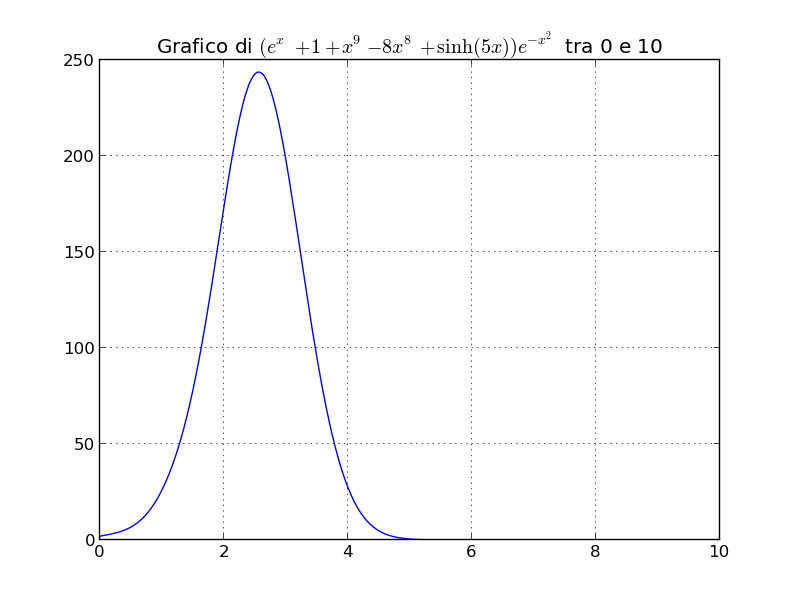
\includegraphics[scale=0.5]{../images/funzione-integranda.png}
\end{center}
\begin{center}
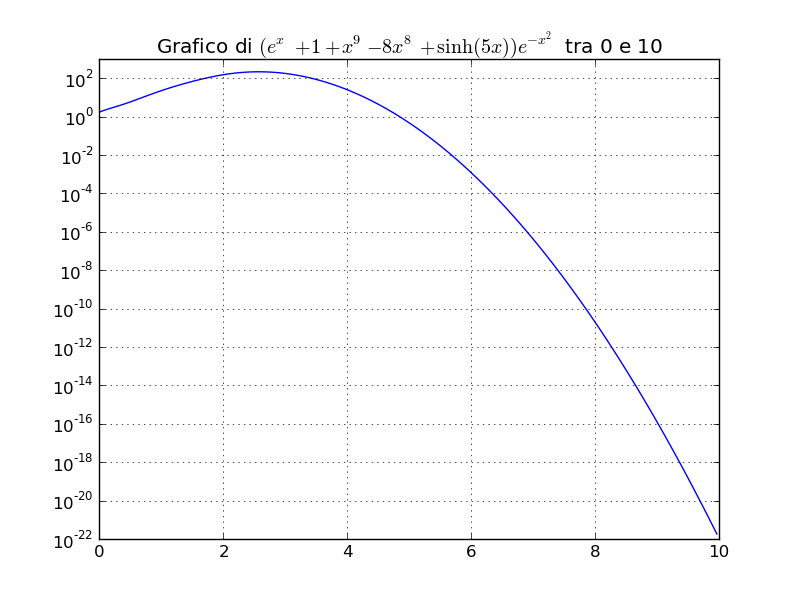
\includegraphics[scale=0.5]{../images/funzione-integranda-log.png}
\end{center}
%\caption{Funzione integranda}
%\end{figure}
Come test delle procedure, integriamo questa funzione tra 1 e 10, e valutiamo il modulo dell'errore rispetto al valore vero dell'integrale (ottenuto mediante procedure di integrazione indipendenti e a precisione arbitraria).

\subsubsection{Errore in funzione del numero di intervalli}
Per aumentare la precisione dei nostri conti senza fare crescere i polinomi utilizzati di grado, possiamo dividere il nostro intervallo di integrazione in $m$ sottointervalli ($m = (b-a)/h$).

Calcolando esplicitamente l'errore in funzione di $m$, si ottengono i seguenti risultati:
\begin{description}
\item[Trapezi] $$\text{Err} \propto \frac{(b-a)^3}{12m^2}\propto\frac{1}{m^2}$$
\item[Simpson] $$\text{Err} \propto \frac{(b-a)^5}{180(2m)^4} \propto\frac{1}{m^4}$$
\item[Quadrature gaussiane] Utilizzando un polinomio di ordine $n$ si ha che $$\text{Err} \propto m\frac{f^{(2n)}(\xi)}{(2n)!}\frac{1}{m^{2n}} \propto\frac{1}{m^{2n-1}}$$
\end{description}

Dapprima svolgiamo il conto con i numeri \texttt{double} e grafichiamo l'andamento dell'errore rispetto al campionamento. Utilizziamo per le quadrature gaussiane polinomi di grado 5.
\begin{center}
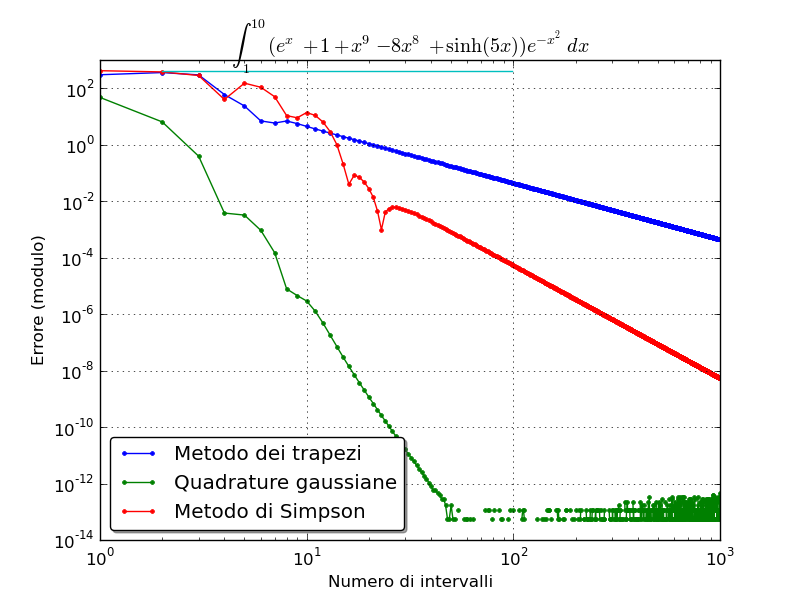
\includegraphics[scale=0.5]{../images/integrali/integralisommaprecisa.png}
\end{center}
Notiamo come la precisione del metodo delle quadrature gaussiane raggiunge quasi subito la precisione macchina, mentre gli altri due metodi impiegano più tempo a convergere.

Utilizziamo, per continuare la nostra analisi, una libreria C (GNU MPFR) per utilizzare dei numeri floating-point a 50 cifre significative, e ripetiamo i risultati con più intervalli.

\begin{center}
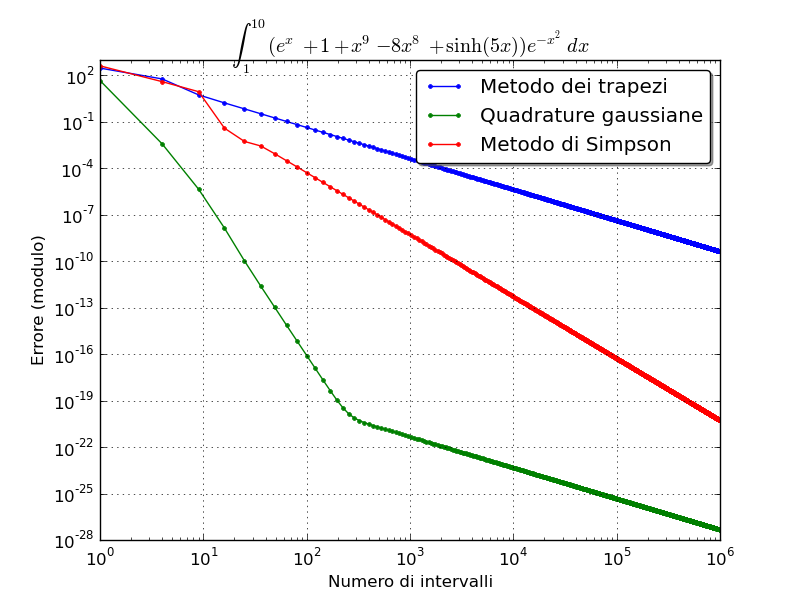
\includegraphics[scale=0.5]{../images/integrali/integralibigprecision-longrun.png}
\end{center}

Notiamo come l'errore sia nel metodo dei trapezi che in quello di Simpson continua a calare come previsto fino a una precisione di $10^{-20}$, oltre la quale entrano in gioco arrotondamenti sconosciuti che limitano la velocità di caduta dell'errore delle quadrature gaussiane.

Eseguendo un fit con una funzione del tipo $y = Ax^{-B}$ per valutare la pendenza delle rette otteniamo i valori:
\begin{description}
\item[Trapezi] $B=2.13 \pm 0.43$
\item[Simpson] $B=4.14 \pm 0.11$
\item[Gauss] $B=8.9 \pm 0.5$
\end{description}

ovvero tutti valori compatibili con la teoria.

\subsection{Conclusioni}

Esistono diversi metodi deterministici per approssimare numericamente integrali analiticamente sconosciuti. Le formule di Newton-Cotes sono strumenti molto potenti nel caso in cui si disponga di campionamenti della funzione equispaziati (caso molto comune in fisica sperimentale). Nel caso, invece, in cui si possa campionare la funzione integranda a piacere, è più conveniente utilizzare le formule di quadratura gaussiana, che arrivano a soluzioni precise molto velocemente.

I risultati ottenuti sono compatibili con le previsioni teoriche.

\section{Integrazione Monte-Carlo}

I metodi per l'integrazione deterministica sono molto efficienti, ma risentono di problemi quando si vogliano adattare a casi multidimensionali.
Un'analisi approfondita degli errori nel caso multidimensionale mostra che la complessità computazionale cresce esponenzialmente con il numero delle dimensioni. Se prima il costo computazionale $N_c$ era proporzionale al numero di intervalli $m$, ora $N_c \propto m^d$, dove $d$ è il numero di dimensioni. Questo ha effetti catastrofici sulla convergenza degli integrali. Ad esempio, nel caso dei trapezi, l'errore diventa:
$$E\propto\frac{1}{N^{\frac{2}{d}}}$$
Ciò è particolarmente problematico per integrali in $10^9$ dimensioni, non rari in Fisica Teorica.

Per ovviare a questo fatto, vengono introdotti i metodi di integrazione Montecarlo, che basano la loro efficacia sul campionamento casuale della funzione. Questi metodi hanno la piacevole caratteristica (derivante da teoremi statistici) di avere un errore sempre proporzionale a $N^{-1/2}$ (con $N$ numero di campionamenti), indipendentemente dal numero di dimensioni in cui si sta operando.

Il teorema su cui si basa la teoria dell'integrazione Monte-Carlo è il teorema del limite centrale, che stabilisce che, date $N$ variabili aleatorie $\{x_i\}$ con distribuzione di probabilità qualsiasi, al limite $N\to\infty$ la variabile somma $y = \sum x_i$ sarà distribuita in modo gaussiano.
In generale allora

\subsection{Ago di Buffon}

\section{Integali di Feynman}

\section{Calcolo di equazioni differenziali}

\end{document}
